\section{Arquitectura capa de tecnología}
{Esta capa, es la capa de arquitectura del proyecto orientada a la tecnología, aquí se define el hardware y el modelo de comunicación que soportara el mínimo necesario para desplegar el producto \cite{archimate}.}

	\subsection{Punto de vista de infraestructura}
	{Permite visualizar los sistemas de software que soportaran la aplicación (sistemas operativos, base de datos, etc) \cite{archimate}.
	\newpage
		
		\textbf{Modelo}\\
		\begin{figure}[H]
			\centering
			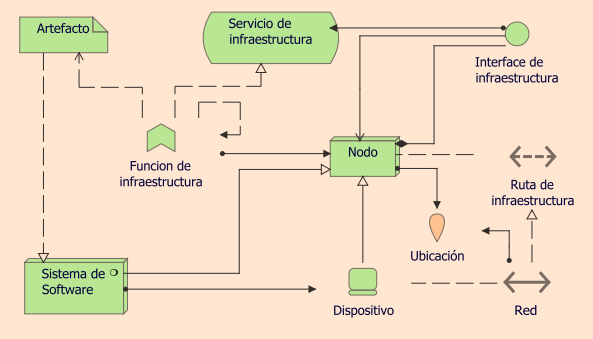
\includegraphics[width=0.7\linewidth]{development/infraestructura.png}
			\caption{Metamodelo de Infraestructura}
		\end{figure}
		\begin{center}
			\textbf{Fuente:} Colosoft E.U: Documento CasoColoSoft.
		\end{center}
		\hfill
	
		\textbf{Caso:} El enfoque de la infraestructura está basado en el sistema operativo Windows y en el motor de base de datos Postgresql, donde serán complementados funcionalmente por sistemas externos como una conexión a internet.
		
		\begin{figure}[H]
			\centering
			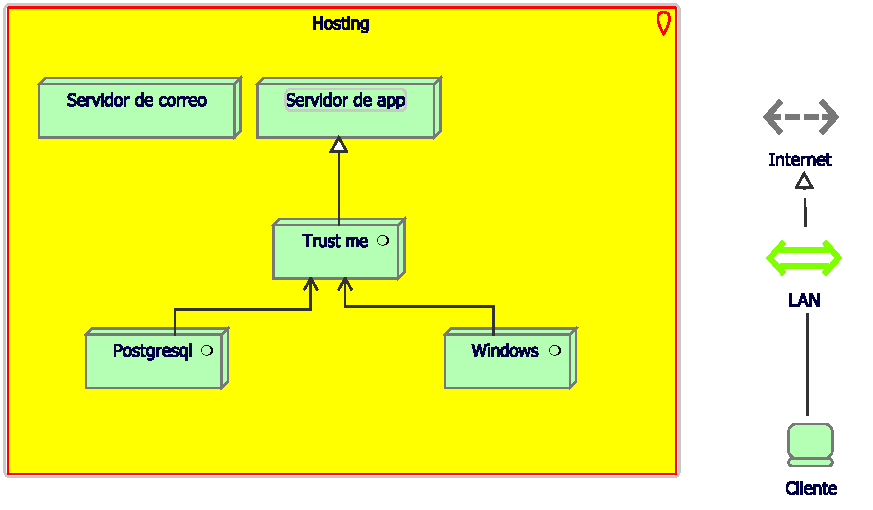
\includegraphics[width=0.8\linewidth]{development/infraestructura.pdf}
			\caption{Infraestructura}
		\end{figure}
		\begin{center}
			\textbf{Fuente:} Propia.
		\end{center}
	}
	
	\subsection{Punto de vista de uso de infraestructura}
	{Muestra el soporte de la infraestructura del software y el hardware, donde se evaluara el rendimiento, la escalabilidad y la usabilidad de la aplicación, permitiendo determinar nuevos requerimientos que solucionen posibles problemas a futuro, garantizando un producto de calidad \cite{archimate}.\\
		
		\textbf{Modelo}\\
		\begin{figure}[H]
			\centering
			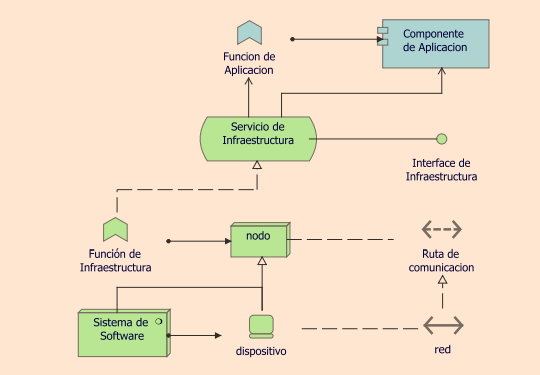
\includegraphics[width=0.8\linewidth]{development/usoinfraestructura.png}
			\caption{Metamodelo de Uso de Infraestructura}
		\end{figure}
		\begin{center}
			\textbf{Fuente:} Colosoft E.U: Documento CasoColoSoft.
		\end{center}
		\hfill \break
		
		\textbf{Caso:} Se da un enfoque de la organización de cada uno de los componentes que se encuentran desplegados dentro de la aplicación WEB, siendo el servidor de la app el nodo principal de estos.
		
		\begin{figure}[H]
			\centering
			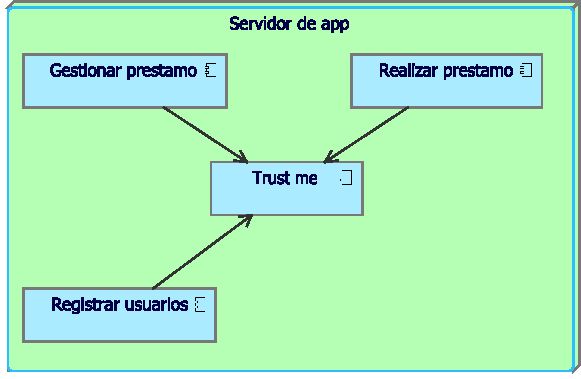
\includegraphics[width=0.8\linewidth]{development/usoinfraestructura.pdf}
			\caption{Uso de Infraestructura}
		\end{figure}
		\begin{center}
			\textbf{Fuente:} Propia.
		\end{center}
		\hfill \break
	}
	
	\subsection{Punto de vista de estructura de información}
	{Muestra la estructura de la información usada en la aplicación en términos de los tipos de datos, son comparables con los modelos tradicionales creados en el desarrollo de la mayoría de los sistemas de información \cite{archimate}.
	\newpage
			
		\textbf{Modelo}\\
		\begin{figure}[H]
			\centering
			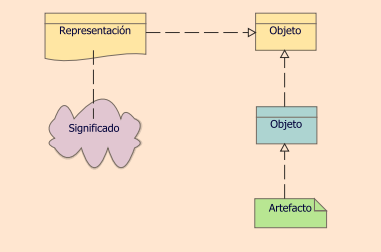
\includegraphics[width=0.8\linewidth]{development/estructurainfo.png}
			\caption{Metamodelo de Estructura de la información}
		\end{figure}
		\begin{center}
			\textbf{Fuente:} Colosoft E.U: Documento CasoColoSoft.
		\end{center}
		\hfill \break
		
		\textbf{Caso:} El objeto principal de la aplicación es un préstamo, el cual se ve influido por la interacción del prestador y el prestatario, dando como resultado la actualización de detalles del préstamo.
		
		\begin{figure}[H]
			\centering
			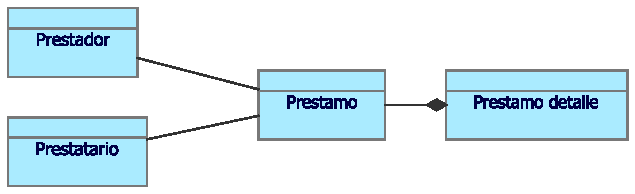
\includegraphics[width=0.8\linewidth]{development/estructurainfo.pdf}
			\caption{Estructura de la información}
		\end{figure}
		\begin{center}
			\textbf{Fuente:} Propia.
		\end{center}
	}
	
	\subsection{Punto de vista de realización del servicio}
	{Es usado para mostrar la utilización de los servicios por los procesos subyacentes, esta crea una estructura sólida que permite la conexión entre el producto del negocio y los procesos del negocio \cite{archimate}.\\
		
		\textbf{Modelo}\\
		\begin{figure}[H]
			\centering
			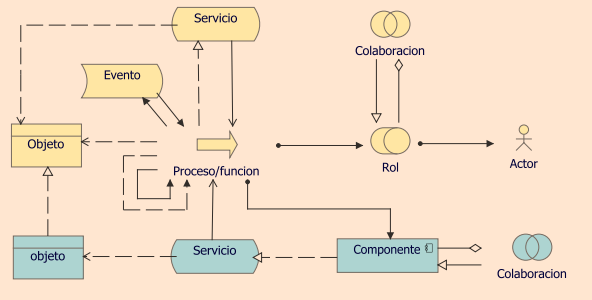
\includegraphics[width=0.8\linewidth]{development/realizacionser.png}
			\caption{Metamodelo de Realización Servicio}
		\end{figure}
		\begin{center}
			\textbf{Fuente:} Colosoft E.U: Documento CasoColoSoft.
		\end{center}
		\hfill \break
		
		\textbf{Caso:} Muestra el proceso del negocio de la arquitectura: la gestión de préstamos, donde el prestador y el prestatario deberán ponerse de acuerdo para conseguir o realizar el mismo.
			
		
		\begin{figure}[H]
			\centering
			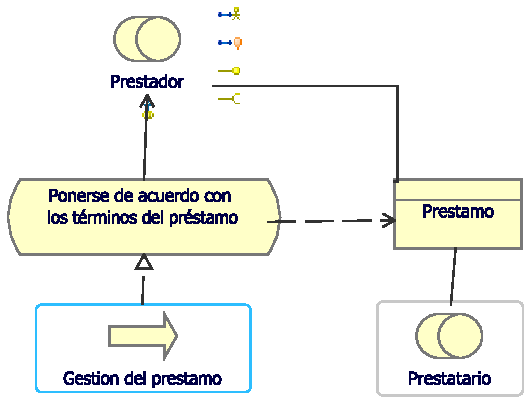
\includegraphics[width=0.8\linewidth]{development/realizacionser.pdf}
			\caption{Realización Servicio}
		\end{figure}
		\begin{center}
			\textbf{Fuente:} Propia.
		\end{center}
	}
	
